\section{Spring Peer Review}


\textbf{Spring Peer review:} 

You will see that this word document allows you to record your name, and that of your reviewer. The owner of the OneNote can then pre-fill in the yellow sections indicating where they think they have shown evidence of particular skills. As this is relatively early in the process there is likely to be more evidence of planning and research, and less of skill development, which is why it only covers the AO1 and AO2 sections of the mark scheme. 
If you are using this document to peer-review a classmate's EP work, add your name and feedback in the green sections. Often it is a good idea to look for what is missing as well as what is present. If you can circle sections of the mark scheme as well as give general feedback that will be helpful. 
Finally, once you have got your EPQ peer review back, make sure you enter some notes and actions for yourself. If you can demonstrate taking and acting on advice it helps to show active project management. 

Peer Marking exercise	

\textbf{Date:} 31/ 1/ 2025 

\textbf{Project topic:} Digitised workflows and human knowledge retention

\textbf{Marker name:} Matthew

\textbf{Task:} use the mark scheme to identify areas where there is no/poor/little evidence being provided. Offer suggestions on how to improve the evidence being provided to better show how the project is being managed. 

\subsection*{AO1: Planning and Research}
\label{Evaluation:SpringPeerReview}
\begin{figure}[H]
\centering
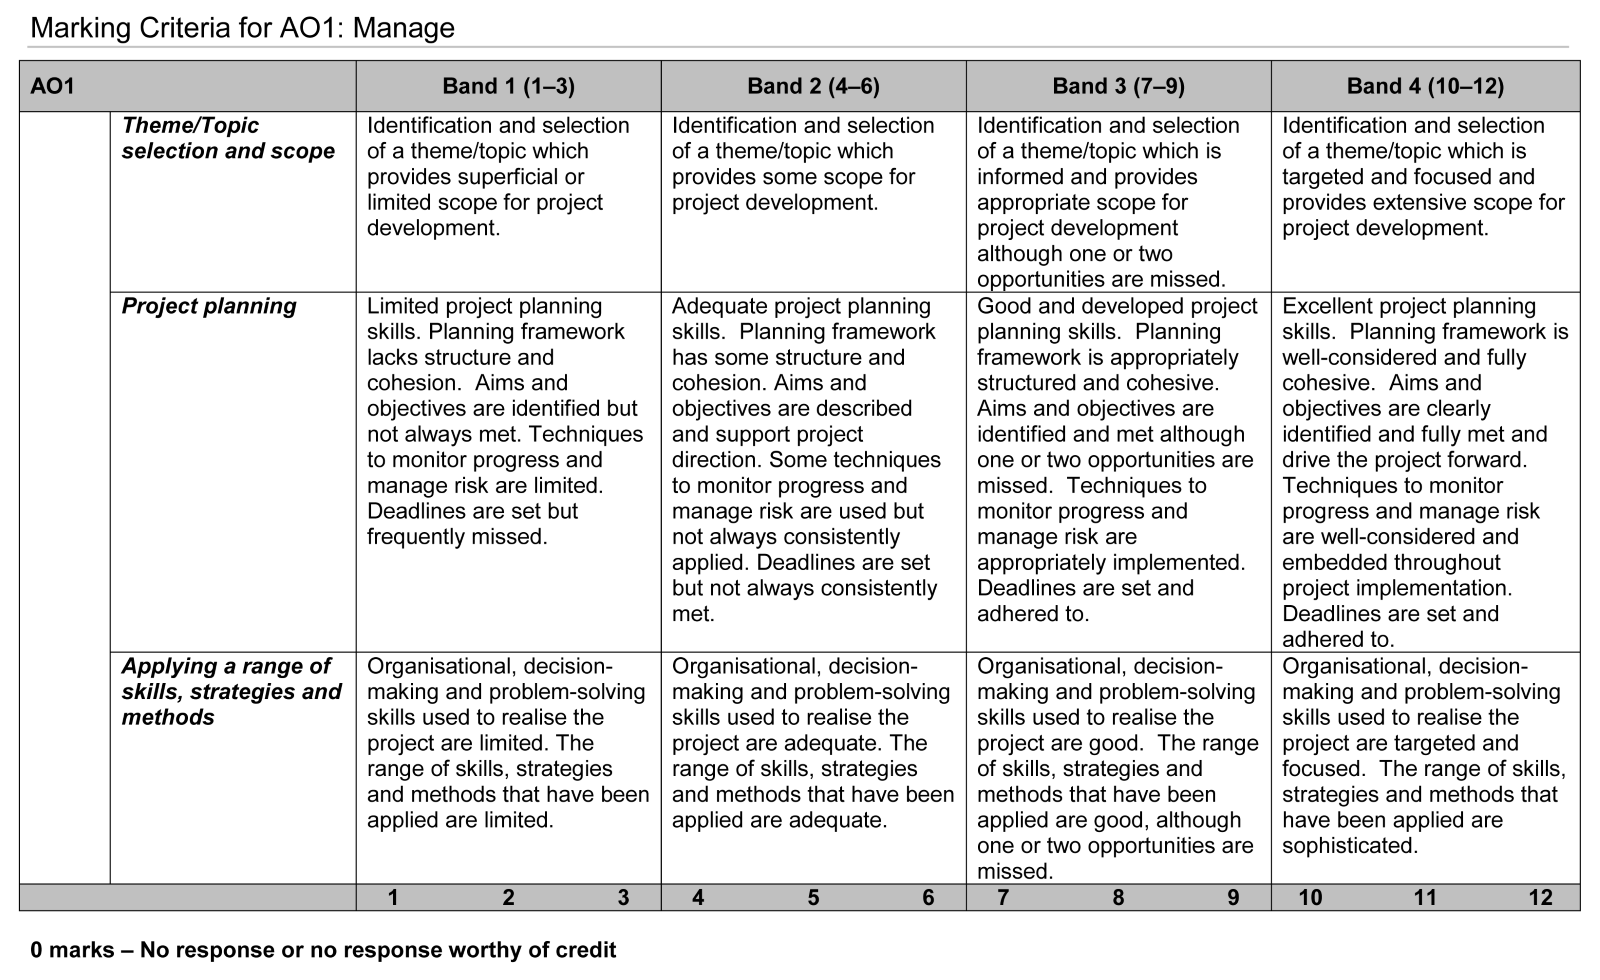
\includegraphics[width=0.8\textwidth]{Evaluation/SpringPeerReview/Media/AO1Criteria.png}
\caption{AO1 Specification}
\end{figure}

\textbf{Reviewer Assessment:}
 10/12 low to mid band 4 due to project planning section which could need a little bit of work due to sections we haven't quite gotten to

\subsection*{AO2: Skill Development}

\begin{figure}[H]
\centering
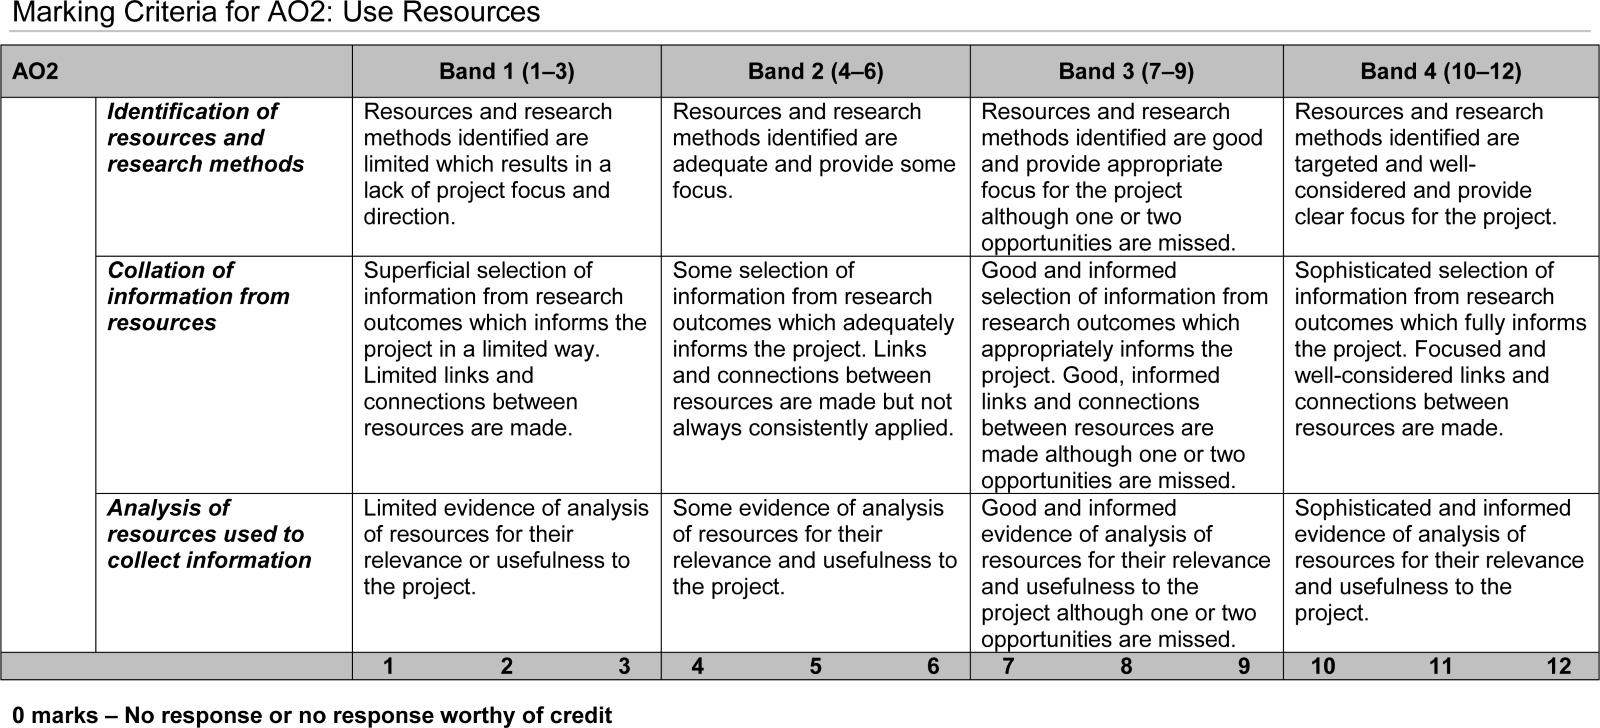
\includegraphics[width=0.8\textwidth]{Evaluation/SpringPeerReview/Media/AO2Criteria.png}
\caption{AO2 Specification}
\end{figure}

\textbf{Reviewer Assessment:}

  11/12 good selection and notes on the research however, could do with summarizing some of the notes in the source evaluation table just to hit the analysis section better.


\subsection*{My Commentary:}
I am very happy with my current progress and feedback and am confident i am heading along the write lines to achieve my target grade. To ensure i continue making strong progress i will update my timeline planning to relfect the feedback given. I will also make time to review my sources more thoroughly in my source evaluation table to pry further into the motivations of the author which will help inform the reliability and relivance of the source.